\begin{figure*}[] 
\centering 
   	
\subfigure[GD values of DTLZ2 with 10-objective]
	{
		\label{fig:dtlz210gdparameter}
		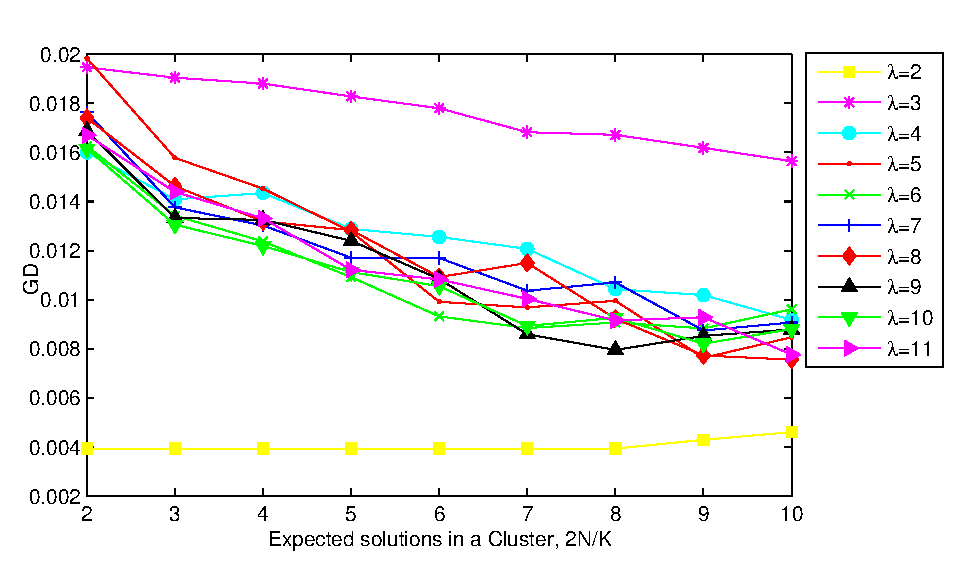
\includegraphics[width=2.50in]{figures/parameter/paramdtlzGD2_10.eps}
	}
~
		\subfigure[IGD values of DTLZ2 with 10-objective]
	{
		\label{fig:dtlz210igdparameter}
		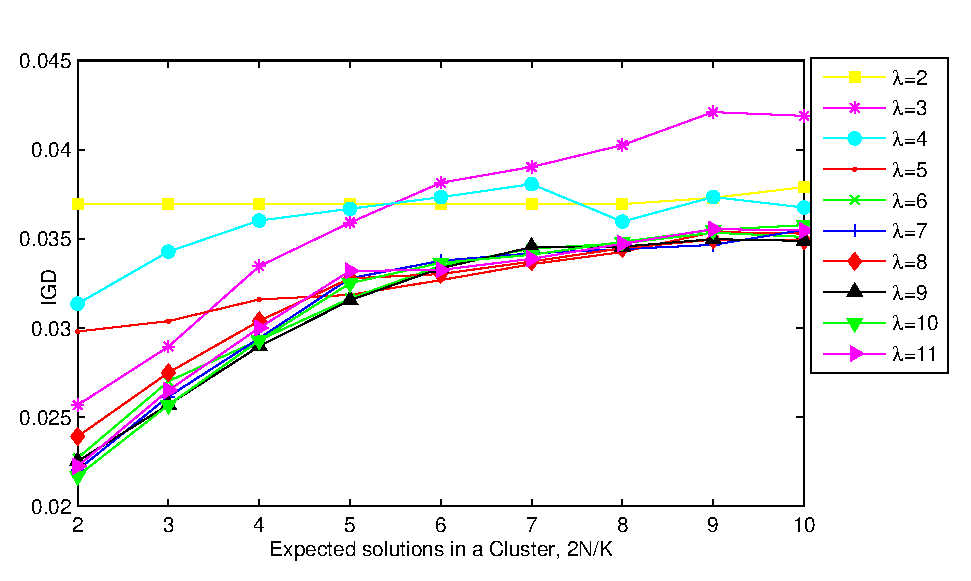
\includegraphics[width=2.50in]{figures/parameter/paramdtlzIGD2_10.eps}
	}
	~
	\subfigure[HV values of DTLZ2 with 10-objective]
	{
		\label{fig:dtlz210hvparameter}
		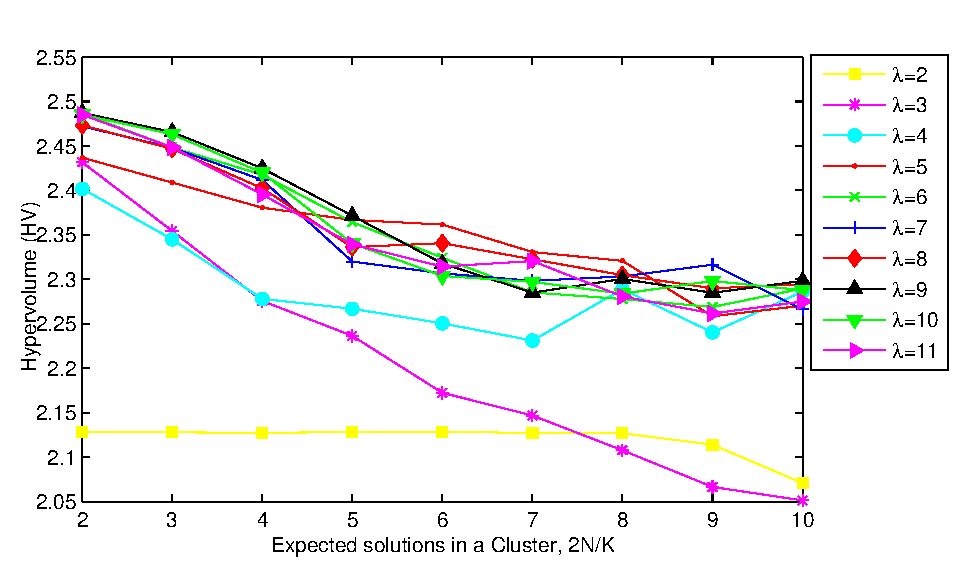
\includegraphics[width=2.50in]{figures/parameter/paramdtlzHV2_10.eps}
	}
\caption{Effect of $\lambda$ and $\chi$ on GD, IGD and HV  performance of $F$-DEA  on the DTLZ2 problem with $10$-objective. %The plots show expected number of solutions in a cluster($\chi$) for a fixed population size $N=250$ vs HV performance for incremental values of $\lambda$ in horizontal line. The stable parameter for $\lambda$ selected as $9,\ 6$ for objective $10,\ 15$ respectively.
}
\label{fig:parametersensitivty}
\end{figure*}
